\begin{quote}
	\textit{``If the chaos of the nineties reflects a radical shift in the paradigms of visual literacy, the final shift away from the Lascaux/Gutenberg tradition of a pre-holographic society, what should we expect from this newer technology, with his promise of discrete encoding and subsequent reconstruction of the full range of sensory perception?''}
\end{quote}
\hfill \textit{Burning Chrome, William Gibson}
\\
\\

%=========================================================================================================

\label{chapter-conclusions}

Introduction goes here.

\begin{figure}[h]
	\begin{center}
		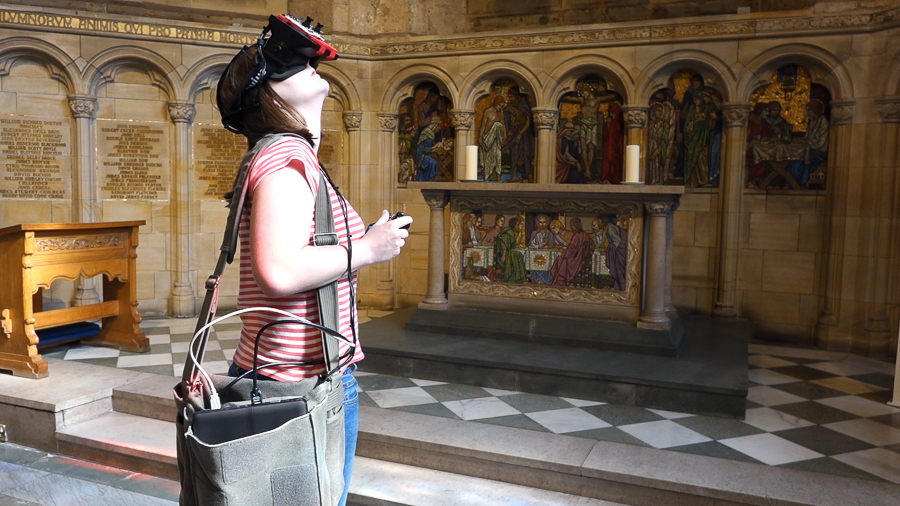
\includegraphics[width=\textwidth]{participant-f-4.jpg}
		\caption{The \textit{Mirrorshades} parallel reality platform in use.}
		\label{participant-f-4.jpg}
	\end{center}	
\end{figure}

%=========================================================================================================

\section{Contributions}

As listed in section \ref{intro-contributions} the contributions of this thesis can be summarized as follows;

\begin{itemize}
	\item The introduction of parallel reality as a new category of alternate reality that allows users to experience two complete environments in tandem \& represents an approach for mitigation of the vacancy problem.
	\item The framing of parallel reality through a thorough investigation \& extension of previous taxonomies that classify \& distinguish alternate reality terminologies.
	\item The creation of the combined Milgram/Waterworth model for visualising alternate reality experiences, including those of parallel reality systems.
	\item Development of a parallel reality platform, dubbed Mirrorshades, that combines new virtual reality hardware with novel indoor positioning technology.
	\item Evaluation of the Mirrorshades platform through user studies of a real world use case study within the realm of cultural heritage, including the application of an established presence questionnaire to parallel reality.
	\item Discussion \& creation of a set of best practices for future parallel reality endeavours.
\end{itemize}

%=========================================================================================================

\section{Future Work}

Gear VR style hardware

%=========================================================================================================

\section{Final Thoughts}

Final quote?

%=========================================================================================================